%%\documentclass[a4paper,12pt,oneside]{llncs}
\documentclass{book}
%\usepackage[right=2cm,left=3cm,top=2cm,bottom=2cm,headsep=0cm]{geometry}

%%%%%%%%%%%%%%%%%%%%%%%%%%%%%%%%%%%%%%%%%%%%%%%%%%%%%%%%%%%
%% Juego de caracteres usado en el archivo fuente: UTF-8
\usepackage{ucs}
\usepackage[utf8x]{inputenc}

%%%%%%%%%%%%%%%%%%%%%%%%%%%%%%%%%%%%%%%%%%%%%%%%%%%%%%%%%%%
%% Juego de caracteres usado en la salida dvi
%% Otra posibilidad: \usepackage{t1enc}
\usepackage[T1]{fontenc}

%%%%%%%%%%%%%%%%%%%%%%%%%%%%%%%%%%%%%%%%%%%%%%%%%%%%%%%%%%%
%% Ajusta maergenes para a4
\usepackage{a4wide}

%%%%%%%%%%%%%%%%%%%%%%%%%%%%%%%%%%%%%%%%%%%%%%%%%%%%%%%%%%%
%% Uso fuente postscript times, para que los ps y pdf queden y pequeños...
\usepackage{times}

%%%%%%%%%%%%%%%%%%%%%%%%%%%%%%%%%%%%%%%%%%%%%%%%%%%%%%%%%%%
%% Posibilidad de hipertexto (especialmente en pdf)
\usepackage{hyperref}

%%%%%%%%%%%%%%%%%%%%%%%%%%%%%%%%%%%%%%%%%%%%%%%%%%%%%%%%%%%
%% Graficos 
\usepackage{graphics,graphicx}

%%%%%%%%%%%%%%%%%%%%%%%%%%%%%%%%%%%%%%%%%%%%%%%%%%%%%%%%%%%
%% Ciertos caracteres "raros"...
\usepackage{latexsym}

%%%%%%%%%%%%%%%%%%%%%%%%%%%%%%%%%%%%%%%%%%%%%%%%%%%%%%%%%%%
%% Matematicas aun más fuertes (american math dociety)
\usepackage{amsmath}

%%%%%%%%%%%%%%%%%%%%%%%%%%%%%%%%%%%%%%%%%%%%%%%%%%%%%%%%%%%
\usepackage{multirow} % para las tablas
\usepackage[spanish,es-tabla]{babel}

%%%%%%%%%%%%%%%%%%%%%%%%%%%%%%%%%%%%%%%%%%%%%%%%%%%%%%%%%%%
%% Fuentes matematicas lo mas compatibles posibles con postscript (times)
%% (Esto no funciona para todos los simbolos pero reduce mucho el tamaño del
%% pdf si hay muchas matamaticas....
\usepackage{mathptm}

%%% VARIOS:
\usepackage{slashbox}
\usepackage{verbatim}
\usepackage{array}
\usepackage{listings}
\usepackage{multirow}
\usepackage{hhline}

%% MARCA DE AGUA
%% Este package de "draft copy" NO funciona con pdflatex
%%\usepackage{draftcopy}
%% Este package de "draft copy" SI funciona con pdflatex
%%%\usepackage{pdfdraftcopy}
%%%%%%%%%%%%%%%%%%%%%%%%%%%%%%%%%%%%%%%%%%%%%%%%%%%%%%%%%%%
%% Indenteacion en español...
\usepackage[spanish]{babel}
\usepackage{Estilos/Apuntes}
\usepackage[svgnames,x11names,table]{xcolor}
\usepackage{listings}
% Para escribir código en C
% \begin{lstlisting}[language=C]
% #include <stdio.h>
% int main(int argc, char* argv[]) {
% puts("Hola mundo!");
% }
% \end{lstlisting}


\title{{\Huge Cableado estructurado}\\\textcolor{White}{ }\\
	\begin{LARGE} 
		GrupoLaboratorio\_2
\end{LARGE}}
\author{Borja Caro Macho\\Alejandro Cuesta Contreras\\Manuel Fernández Rosado\\Francisco Javier Jiménez Vázquez\\Arantzazu Otal Alberro\\Francisco Javier Pérez Sánchez\\Juan Pedro Rodríguez Gracia\\Jesús Rodríguez Heras\\Gabriel Fernando Sánchez Reina\\José Antonio Torres Leal}



\begin{document}
	\maketitle
	\thispagestyle{empty}
	\newpage
	\textcolor{White}{ }
	\newpage
	\textcolor{White}{.}
%	\newpage
	\thispagestyle{empty}
	
	\begin{table}[htbp]
		\begin{center}
			\begin{tabular}{|l|p{0.6cm}|p{0.6cm}|p{0.6cm}|p{0.6cm}|p{0.6cm}|p{0.6cm}|p{0.6cm}|p{0.6cm}|}
				\rowcolor[gray]{0.8}
				\hline
				\textbf{Integrantes} & \rotatebox{90}{\textbf{Pregunta 1 }} & \rotatebox{90}{\textbf{Pregunta 2 }} & \rotatebox{90}{\textbf{Pregunta 3 }} & \rotatebox{90}{\textbf{Pregunta 4 }} & \rotatebox{90}{\textbf{Pregunta 5 }} & \rotatebox{90}{\textbf{Pregunta 6 }} & \rotatebox{90}{\textbf{Pregunta 7 }} & \rotatebox{90}{\textbf{Pregunta 8 }} \\
				\hline 
				Borja Caro Macho &  & &&&&&&\\ \hline
				Alejandro Cuesta Contreras &  & &&&&&&\\ \hline
				Manuel \newline Fernández Rosado &  & &&&&&&\\ \hline
				Francisco Javier \newline Jiménez Vázquez &  & &&&&&&\\ \hline
				Arantzazu Otal Alberro &  & &&&&&&\\ \hline	
				Francisco Javier Pérez Sánchez &  & &&&&&&\\ \hline
				Juan Pedro Rodríguez Gracia &  & &&&&&&\\ \hline
				Jesús \newline Rodríguez Heras &  & &&&&&&\\ \hline
				Gabriel \newline Fernando Sánchez Reina &  & &&&&&&\\ \hline
				José \newline Antonio \newline Torres Leal &  & &&&&&&\\ \hline
			\end{tabular}
		\end{center}
	\end{table}
	Coordinador: José Antonio Torres Leal.\\
	Ponente 1: Alejandro Cuesta Contreras.\\
	Ponente 2: Juan Pedro Rodríguez Gracia.\\
	
	Pregunta 1:.................................................................................................................................................................................\\
		
	Pregunta 2:.................................................................................................................................................................................\\
		
	Pregunta 3:.................................................................................................................................................................................\\
		
	Pregunta 4:.................................................................................................................................................................................\\
		
	Pregunta 5:.................................................................................................................................................................................\\
		
	Pregunta 6:.................................................................................................................................................................................\\
		
	Pregunta 7:.................................................................................................................................................................................\\
		
	Pregunta 8:.................................................................................................................................................................................
	
	\newpage
	\thispagestyle{empty}
	
	\textcolor{White}{ }
	\newpage
	\thispagestyle{empty}
	

	
	\begin{table}[htbp]
		\begin{center}
			\begin{tabular}{|c|c|c|}
				\rowcolor[gray]{0.8}
				\hline
				\textbf{Conceptos a valorar} & \textbf{Puntuación máxima} & \textbf{Puntuación otorgada} \\
				\hline 
				Contenido del dossier claro y detallado & 3 puntos  & \\ \hline
				Maquetación/Formato del dossier & 1 punto & \\ \hline
				Ponente 1 & 1 punto & \\ \hline
				Ponente 2 & 1 punto & \\ \hline
				Preguntas formuladas & 4 puntos & \\ \hline	
				Puntuación total & \multicolumn{2}{|c|}{\textcolor{White}{ }}\\ \hline
			\end{tabular}
		\end{center}
	\end{table}
	\newpage
	\thispagestyle{empty}
	\textcolor{White}{ }
	\newpage
	\tableofcontents
	\newpage
	
	\chapter{Plano de cableado horizontal}
\section{Planta baja}
\begin{center}
	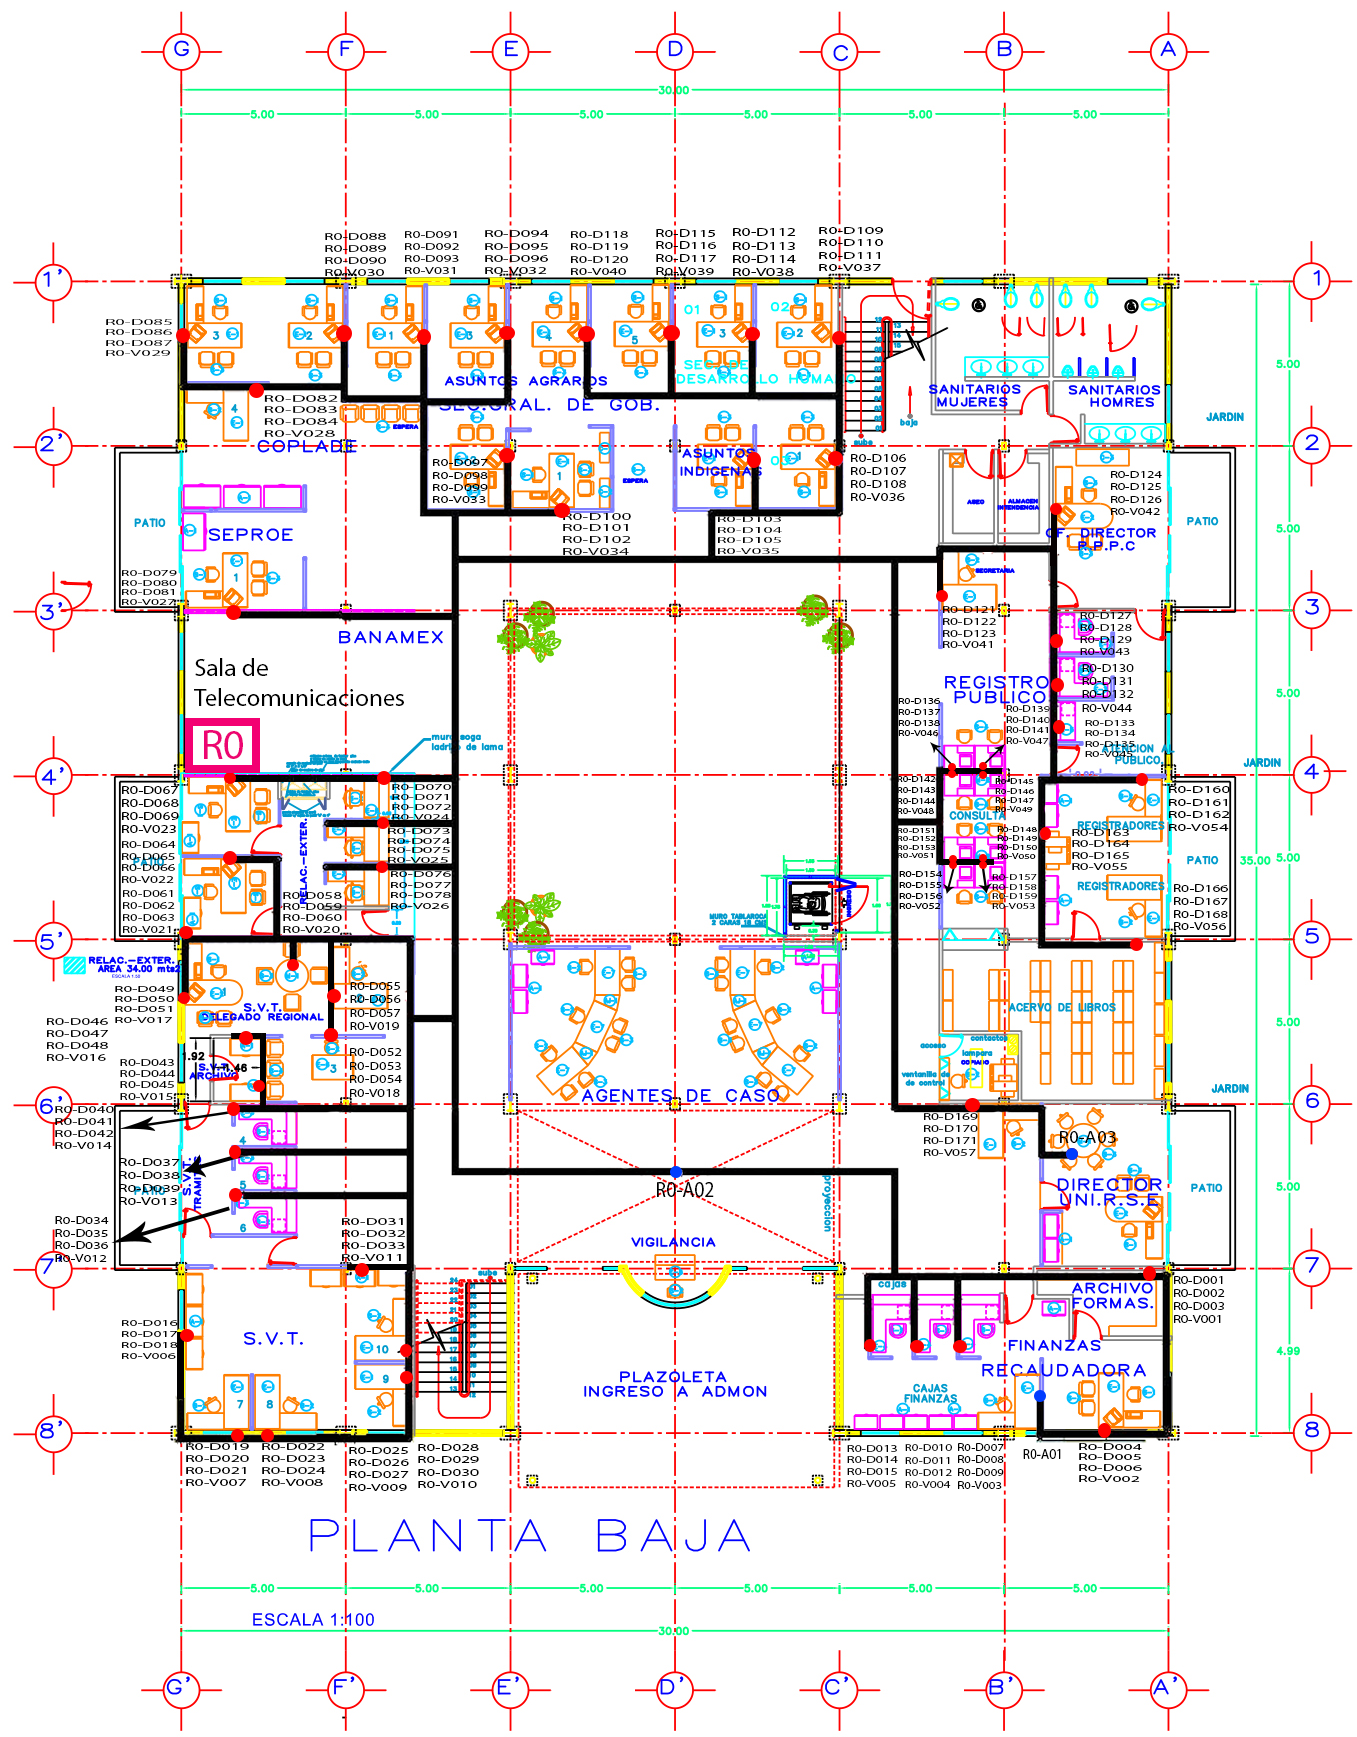
\includegraphics[scale=1.01]{CHPB.png}
\end{center}
\subsection{Salas de telecomunicaciones y de equipamiento}
La sala de telecomunicaciones y de equipamiento se encuentra en la sala nombrada como ``BANAMEX'', que es donde se encontraría el rack 0, el cual hace las funciones de rack de planta y de edificio.

\subsection{Distribuidores etiquetados}
El distribuidor de esta planta se encuentra enumerado como ``R0'' (Rack 0). Las nomenclaturas usadas en el etiquetado han seguido las siguientes normas:
\begin{itemize}
	\item \textbf{Datos. R0-DXXX:} R0 hace referencia al distribuidor de planta baja y XXX es el número de la toma de datos a la cual está conectada.
	\item \textbf{Voz. R0-VXXX:} R0 vuelve a hacer referencia al distribuidor de planta baja y XXX es el número de la toma de voz a al cual está conectada.
	\item \textbf{Puntos de acceso. R0-AXX:} R0 es de nuevo el distribuidor de planta baja y XX es el número de la toma de datos a la cual está conectado el punto de acceso.
\end{itemize}

\subsection{Tomas de comunicaciones etiquetadas instaladas en cada sala}
En cuanto a las tomas de comunicaciones de esta planta, encontramos 171 tomas de datos, 57 tomas de voz y 3 puntos de acceso distribuidos por toda la planta baja.

\newpage
\section{Planta alta}
\begin{center}
	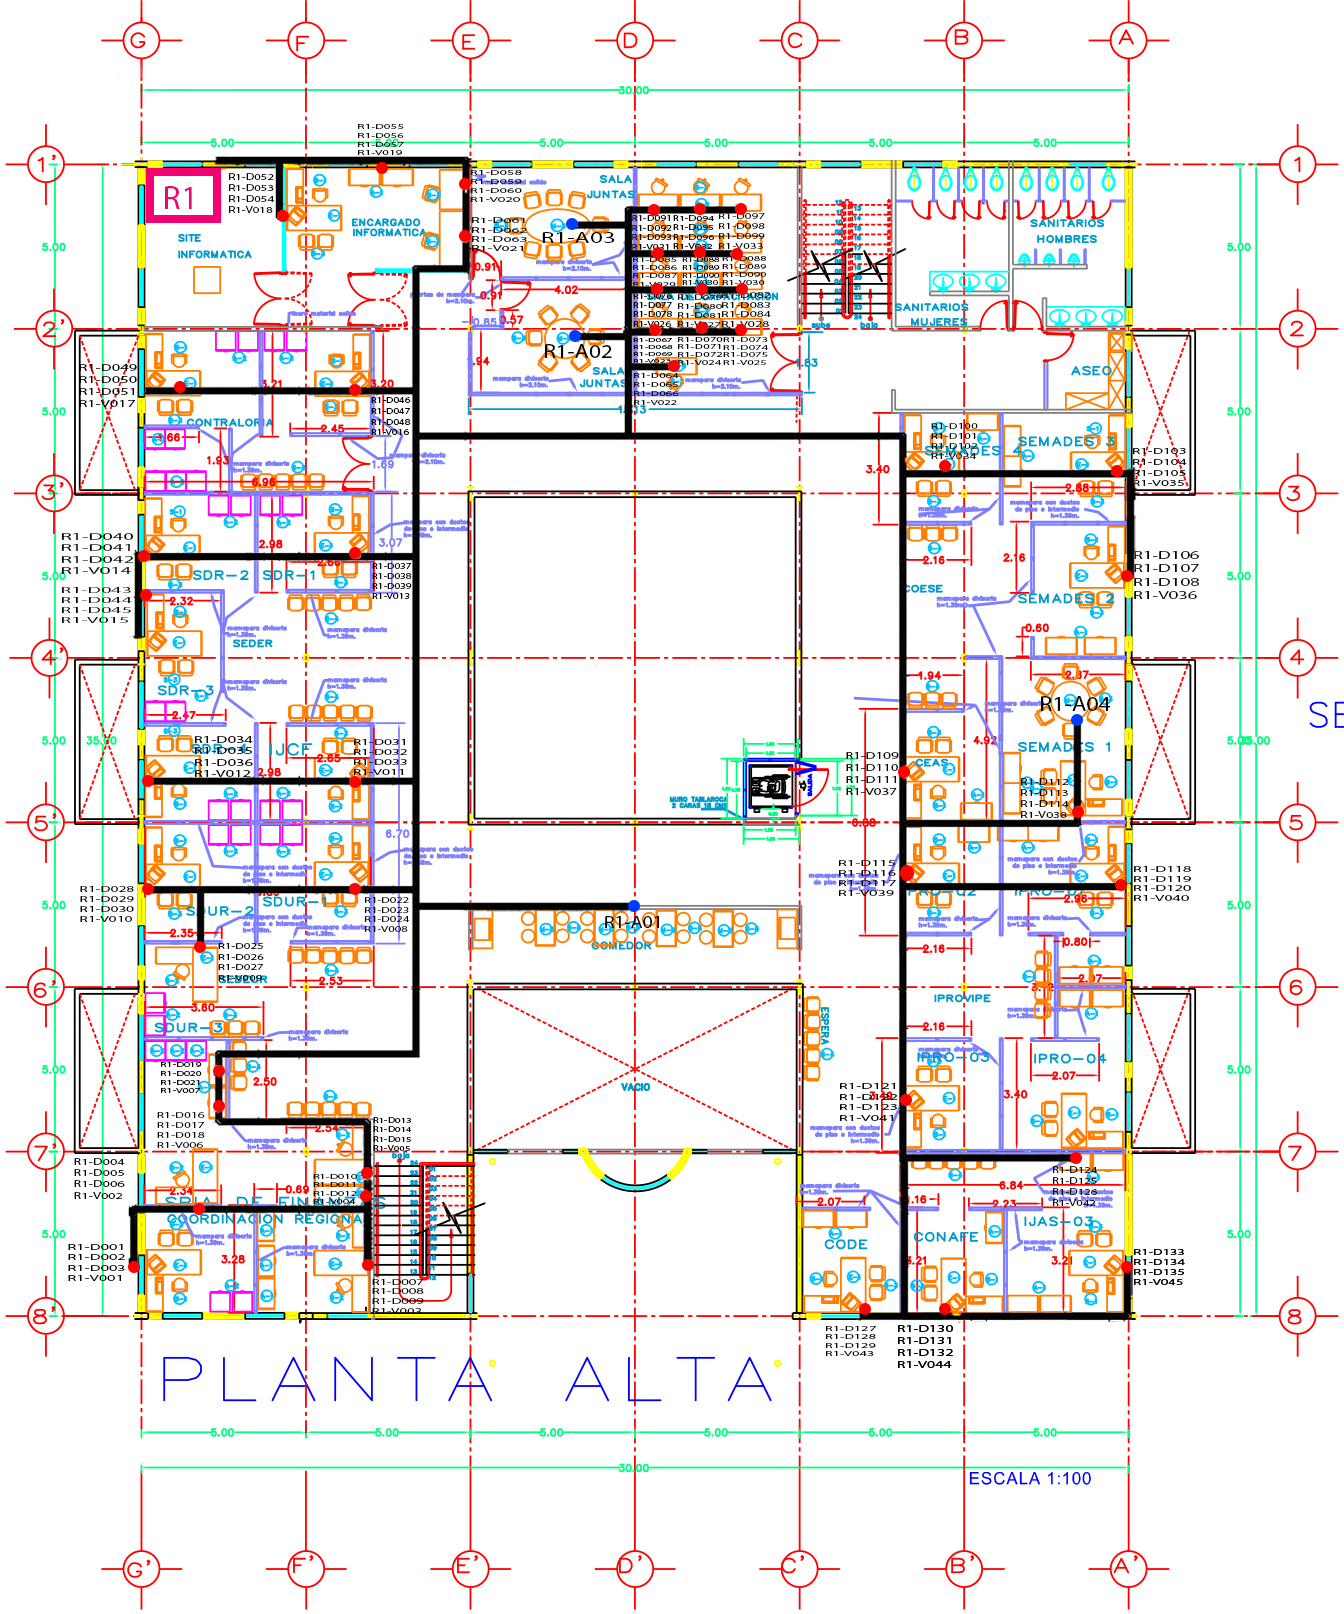
\includegraphics[scale=1.3]{CHPA.png}
\end{center}
\subsection{Salas de telecomunicaciones y de equipamiento}
La sala de telecomunicaciones y de equipamiento se encuentra en la sala nombrada como ``SITE INFORMÁTICA'' que es donde se encontraría el rack 1, el cual hace la función de rack de planta.

\subsection{Distribuidores etiquetados}
El distribuidor de esta planta se encuentra enumerado como ``R1'' (Rack 1). Las nomenclaturas usadas en el etiquetado han seguido las mismas normas que en la planta baja.

\subsection{Tomas de comunicaciones etiquetadas instaladas en cada sala}
En cuanto a las tomas de comunicaciones de esta planta, encontramos 135 tomas de datos, 45 tomas de voz y 4 puntos de acceso distribuidos por toda la planta alta.

	
	\chapter{Distribuidores}
En este capítulo vamos a describir los componentes de los distribuidores de ambas plantas indicando su nombre, la capa OSI en la que se encuentra, la altura física del dispositivo en el distribuidor (medido en U, donde 1U = 1,75 pulgadas = 4,445 centímetros), el número de puertos, el estándar que sigue, el etiquetado, el tipo de conector y la categoría de dicho conector.
\section{Planta baja. RACK 0}
En la siguiente tabla podremos ver detalladamente cada uno de los dispositivos que va a contener el distribuidor de la planta baja con las características anteriormente señaladas.
	\begin{table}[htbp]
	\centering	
	\begin{tabular}{|p{2.5cm}|p{1.6cm}|llllll}
		\hhline{|-|-|}
		\cellcolor[HTML]{CBCEFB}{\textbf{Etiqueta del distribuidor:}}      & R0                  						 &                                      &                                          &                                        &                                             &                                                &                                         \\
		\hhline{|-|-|} 
		\cellcolor[HTML]{CBCEFB}{\textbf{Altura mínima del distribuidor:}} & 26U                  						 &                                      &                                          &                                        &                                             &                                                &                                         \\
		\hhline{|-|-|}
		\cellcolor[HTML]{CBCEFB}{\textbf{Ubicación:}}                      & Sala de telecomunicaciones                  &                                      &                                          &                                        &                                             &                                                &                                         \\
		\hline
		\multicolumn{1}{|c|}{\textbf{Dispositivo}}                     	   & \multicolumn{1}{c|}{\textbf{Capa OSI}} 	 & \multicolumn{1}{c|}{\textbf{Altura}} & \multicolumn{1}{p{1.6cm}|}{\textbf{Nº Puertos}} & \multicolumn{1}{c|}{\textbf{Estándar}} & \multicolumn{1}{p{1.5cm}|}{\textbf{TAT Etiquetas}} & \multicolumn{1}{c|}{\textbf{Tipo de conector}} & \multicolumn{1}{c|}{\textbf{Categoría}} \\
		\hline
		Switch CISCO Catalyst 2960S                                        & \multicolumn{1}{c|}{2}                      & \multicolumn{1}{c|}{1U}              & \multicolumn{1}{p{1.6cm}|}{48 + 4 Fibra Óptica} & \multicolumn{1}{c|}{IEEE 802.3at}      & \multicolumn{1}{p{1.6cm}|}{R0-D001 a R0-D048 (SW-1-R0)} & \multicolumn{1}{c|}{RJ-45 Hembra}              & \multicolumn{1}{c|}{}                   \\ \hline
		Patch Panel Siemon                                                 & \multicolumn{1}{c|}{1}                      & \multicolumn{1}{c|}{2U}              & \multicolumn{1}{c|}{48}                  & \multicolumn{1}{c|}{}                  & \multicolumn{1}{p{1.6cm}|}{R0-D001 a R0-D048}           & \multicolumn{1}{c|}{GG-45 Hembra}              & \multicolumn{1}{c|}{7a}                  \\ \hline
		Switch CISCO Catalyst 2960S                                        & \multicolumn{1}{c|}{2}                      & \multicolumn{1}{c|}{1U}              & \multicolumn{1}{p{1.2cm}|}{48 + 4 Fibra Óptica} & \multicolumn{1}{c|}{IEEE 802.3at}      & \multicolumn{1}{p{1.6cm}|}{R0-D049 a R0-D096 (SW-2-R0)} & \multicolumn{1}{c|}{RJ-45 Hembra}              & \multicolumn{1}{c|}{}                   \\ \hline
		Patch Panel Siemon                                                 & \multicolumn{1}{c|}{1}                      & \multicolumn{1}{c|}{2U}              & \multicolumn{1}{c|}{48}                  & \multicolumn{1}{c|}{}                  & \multicolumn{1}{p{1.6cm}|}{R0-D049 a R0-D096}           & \multicolumn{1}{c|}{GG-45 Hembra}              & \multicolumn{1}{c|}{7a}                  \\ \hline
		Switch CISCO Catalyst 2960S                                        & \multicolumn{1}{c|}{2}                      & \multicolumn{1}{c|}{1U}              & \multicolumn{1}{p{1.2cm}|}{48 + 4 Fibra Óptica} & \multicolumn{1}{c|}{IEEE 802.3at}      & \multicolumn{1}{p{1.6cm}|}{R0-D097 a R0-D144 (SW-3-R0)} & \multicolumn{1}{c|}{RJ-45 Hembra}              & \multicolumn{1}{c|}{}                   \\ \hline
		Patch Panel Siemon                                                 & \multicolumn{1}{c|}{1}                      & \multicolumn{1}{c|}{2U}              & \multicolumn{1}{c|}{48}                  & \multicolumn{1}{c|}{}                  & \multicolumn{1}{p{1.6cm}|}{R0-D097 a R0-D144}           & \multicolumn{1}{c|}{GG-45 Hembra}              & \multicolumn{1}{c|}{7a}                  \\ \hline
		Switch CISCO Catalyst 2960S                                        & \multicolumn{1}{c|}{2}                      & \multicolumn{1}{c|}{1U}              & \multicolumn{1}{p{1.2cm}|}{48 + 4 Fibra Óptica} & \multicolumn{1}{c|}{IEEE 802.3at}      & \multicolumn{1}{p{1.6cm}|}{R0-D145 a R0-D193 R0-A01 a R0-A03 (SW-4-R0)} & \multicolumn{1}{c|}{RJ-45 Hembra}              & \multicolumn{1}{c|}{}                   \\ \hline
		Patch Panel Siemon                                                 & \multicolumn{1}{c|}{1}                      & \multicolumn{1}{c|}{2U}              & \multicolumn{1}{c|}{48}                  & \multicolumn{1}{c|}{}                  & \multicolumn{1}{p{1.6cm}|}{R0-D145 a R0-D193}           & \multicolumn{1}{c|}{GG-45 Hembra}              & \multicolumn{1}{c|}{7a}                  \\ \hline
		Switch CISCO Catalyst 2960S                                        & \multicolumn{1}{c|}{2}                      & \multicolumn{1}{c|}{1U}              & \multicolumn{1}{p{1.2cm}|}{48 + 4 Fibra Óptica} & \multicolumn{1}{c|}{IEEE 802.3at}      & \multicolumn{1}{p{1.6cm}|}{R0-D194 a R0-D242 (SW-5-R0)} & \multicolumn{1}{c|}{RJ-45 Hembra}              & \multicolumn{1}{c|}{}                   \\ \hline
		Router CISCO 2811                                                  & \multicolumn{1}{c|}{3}                      & \multicolumn{1}{c|}{2U}              & \multicolumn{1}{p{1.2cm}|}{2 Fibra (Modular)}   & \multicolumn{1}{c|}{IEEE 802.3af}      & \multicolumn{1}{c|}{(RE)}                        & \multicolumn{1}{c|}{RJ-45 Hembra}              & \multicolumn{1}{c|}{}                   \\ \hline
		Patch Panel de voz Telco                                           & \multicolumn{1}{c|}{1}                      & \multicolumn{1}{c|}{2U}              & \multicolumn{1}{c|}{48}                  & \multicolumn{1}{c|}{EIA/TIA-568}       & \multicolumn{1}{p{1.6cm}|}{R0-V001 a R0-V048}           & \multicolumn{1}{c|}{RJ-45 Hembra}              & \multicolumn{1}{c|}{3}                  \\ \hline
		Patch Panel de voz Telco                                           & \multicolumn{1}{c|}{1}                      & \multicolumn{1}{c|}{2U}              & \multicolumn{1}{c|}{48}                  & \multicolumn{1}{c|}{EIA/TIA-568}       & \multicolumn{1}{p{1.6cm}|}{R0-V049 a R0-V057}           & \multicolumn{1}{c|}{RJ-45 Hembra}              & \multicolumn{1}{c|}{3}                  \\ \hline
		Centralita Nexspan A5000 2XS                                        &                            	   	 		 & \multicolumn{1}{c|}{4U}              & \multicolumn{1}{c|}{112}                 & \multicolumn{1}{c|}{}                  & \multicolumn{1}{c|}{}                            & \multicolumn{1}{c|}{RJ-45 Hembra}              & \multicolumn{1}{c|}{}                   \\ \hline
		Cablematic RE11                                                    &                           					 & \multicolumn{1}{c|}{1U}              & \multicolumn{1}{c|}{}                    & \multicolumn{1}{c|}{}                  & \multicolumn{1}{c|}{}                            & \multicolumn{1}{c|}{}                          & \multicolumn{1}{c|}{}                   \\ \hline
		SAI Lapara Serie On-Rack                                           &                          				     & \multicolumn{1}{c|}{2U}              & \multicolumn{1}{c|}{3}                   & \multicolumn{1}{c|}{}                  & \multicolumn{1}{c|}{}                            & \multicolumn{1}{c|}{RJ-45 Hembra}              & \multicolumn{1}{c|}{}                   \\ \hline
		
	\end{tabular}
\end{table}

\newpage

\section{Planta alta. RACK 1}
En la siguiente tabla podremos ver detalladamente cada uno de los dispositivos que va a contener el distribuidor de la planta alta.

\begin{table}[htbp]
	\centering	
	\begin{tabular}{|p{2.5cm}|p{1.6cm}|llllll}
		\hhline{|-|-|}
		\cellcolor[HTML]{CBCEFB}{\textbf{Etiqueta del distribuidor:}}      & R1                  						 &                                      &                                          &                                        &                                             &                                                &                                         \\
		\hhline{|-|-|} 
		\cellcolor[HTML]{CBCEFB}{\textbf{Altura mínima del distribuidor:}} & 15U                  						 &                                      &                                          &                                        &                                             &                                                &                                         \\
		\hhline{|-|-|}
		\cellcolor[HTML]{CBCEFB}{\textbf{Ubicación:}}                      & Site Informática                  			 &                                      &                                          &                                        &                                             &                                                &                                         \\
		\hline
		\multicolumn{1}{|c|}{\textbf{Dispositivo}}                     	   & \multicolumn{1}{c|}{\textbf{Capa OSI}} 	 & \multicolumn{1}{c|}{\textbf{Altura}} & \multicolumn{1}{c|}{\textbf{Nº Puertos}} & \multicolumn{1}{c|}{\textbf{Estándar}} & \multicolumn{1}{p{1.6cm}|}{\textbf{TAT Etiquetas}} & \multicolumn{1}{c|}{\textbf{Tipo de conector}} & \multicolumn{1}{c|}{\textbf{Categoría}} \\
		\hline
		Switch CISCO Catalyst 2960S                                        & \multicolumn{1}{c|}{2}                      & \multicolumn{1}{c|}{1U}              & \multicolumn{1}{p{1.2cm}|}{48 + 4 Fibra Óptica} & \multicolumn{1}{c|}{IEEE 802.3at}      & \multicolumn{1}{p{1.6cm}|}{R1-D001 a R1-D048 (SW-1-R1)} & \multicolumn{1}{c|}{RJ-45 Hembra}              & \multicolumn{1}{c|}{}                   \\ \hline
		Patch Panel Siemon                                                 & \multicolumn{1}{c|}{1}                      & \multicolumn{1}{c|}{2U}              & \multicolumn{1}{c|}{48}                  & \multicolumn{1}{c|}{}                  & \multicolumn{1}{p{1.6cm}|}{R1-D001 a R1-D048}           & \multicolumn{1}{c|}{GG-45 Hembra}              & \multicolumn{1}{c|}{7a}                  \\ \hline
		Switch CISCO Catalyst 2960S                                        & \multicolumn{1}{c|}{2}                      & \multicolumn{1}{c|}{1U}              & \multicolumn{1}{p{1.2cm}|}{48 + 4 Fibra Óptica} & \multicolumn{1}{c|}{IEEE 802.3at}      & \multicolumn{1}{p{1.6cm}|}{R1-D049 a R1-D096 (SW-2-R1)} & \multicolumn{1}{c|}{RJ-45 Hembra}              & \multicolumn{1}{c|}{}                   \\ \hline
		Patch Panel Siemon                                                 & \multicolumn{1}{c|}{1}                      & \multicolumn{1}{c|}{2U}              & \multicolumn{1}{c|}{48}                  & \multicolumn{1}{c|}{}                  & \multicolumn{1}{p{1.6cm}|}{R1-D049 a R1-D096}           & \multicolumn{1}{c|}{GG-45 Hembra}              & \multicolumn{1}{c|}{7a}                  \\ \hline
		Switch CISCO Catalyst 2960S                                        & \multicolumn{1}{c|}{2}                      & \multicolumn{1}{c|}{1U}              & \multicolumn{1}{p{1.2cm}|}{48 + 4 Fibra Óptica} & \multicolumn{1}{c|}{IEEE 802.3at}      & \multicolumn{1}{p{1.6cm}|}{R1-D097 a R1-D142 R1-A01 a R1-A04 (SW-3-R1)} & \multicolumn{1}{c|}{RJ-45 Hembra}              & \multicolumn{1}{c|}{}                   \\ \hline
		Patch Panel Siemon                                                 & \multicolumn{1}{c|}{1}                      & \multicolumn{1}{c|}{2U}              & \multicolumn{1}{c|}{48}                  & \multicolumn{1}{c|}{}                  & \multicolumn{1}{p{1.6cm}|}{R1-D097 a R1-D142}           & \multicolumn{1}{c|}{GG-45 Hembra}              & \multicolumn{1}{c|}{7a}                  \\ \hline
		Switch CISCO Catalyst 2960S                                        & \multicolumn{1}{c|}{2}                      & \multicolumn{1}{c|}{1U}              & \multicolumn{1}{p{1.2cm}|}{48 + 4 Fibra Óptica} & \multicolumn{1}{c|}{IEEE 802.3at}      & \multicolumn{1}{p{1.6cm}|}{R0-D143 a R0-D191 (SW-4-R1)} & \multicolumn{1}{c|}{RJ-45 Hembra}              & \multicolumn{1}{c|}{}                   \\ \hline
		Patch Panel de voz Telco                                           & \multicolumn{1}{c|}{1}                      & \multicolumn{1}{c|}{2U}              & \multicolumn{1}{c|}{48}                  & \multicolumn{1}{c|}{EIA/TIA-568}       & \multicolumn{1}{p{1.6cm}|}{R1-V001 a R1-V045}           & \multicolumn{1}{c|}{RJ-45 Hembra}              & \multicolumn{1}{c|}{3}                  \\ \hline
		Cablematic RE11                                                    &                           					 & \multicolumn{1}{c|}{1U}              & \multicolumn{1}{c|}{}                    & \multicolumn{1}{c|}{}                  & \multicolumn{1}{c|}{}                            & \multicolumn{1}{c|}{}                          & \multicolumn{1}{c|}{}                   \\ \hline
		SAI Lapara Serie On-Rack                                           &                          				     & \multicolumn{1}{c|}{2U}              & \multicolumn{1}{c|}{3}                   & \multicolumn{1}{c|}{}                  & \multicolumn{1}{c|}{}                            & \multicolumn{1}{c|}{RJ-45 Hembra}              & \multicolumn{1}{c|}{}                   \\ \hline
		
	\end{tabular}
\end{table}
	
	%Doc3
\chapter{Planificación}
%Esto lo hace Gabri con un diagrama de Gantt
En el siguiente diagrama de Gantt podemos observar la planificación del proyecto desde su inicio hasta su final:
\begin{center}
	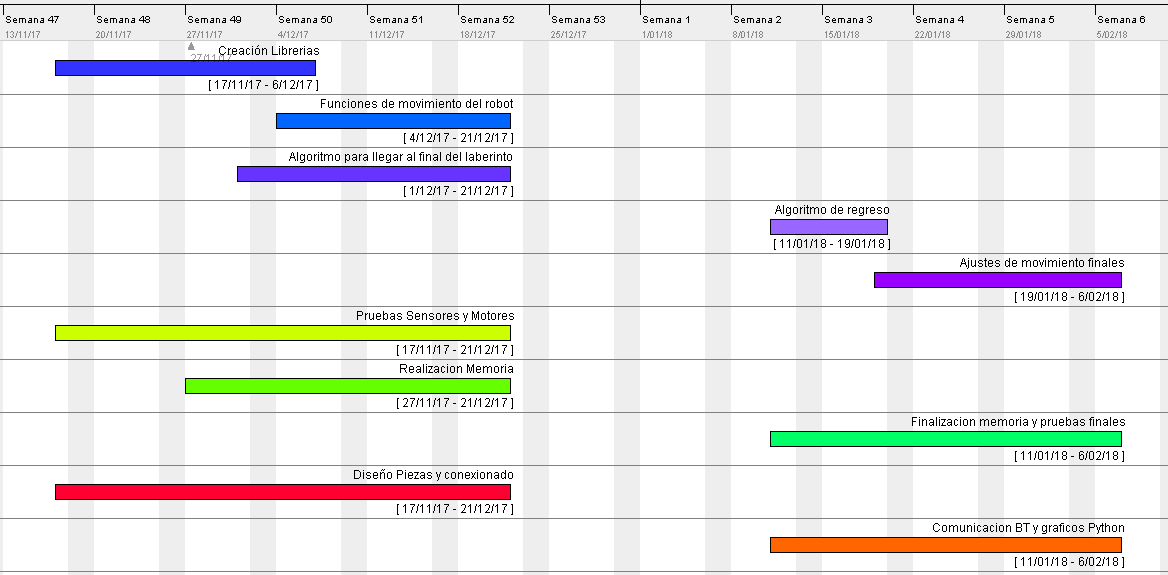
\includegraphics[scale=0.55]{Gant.png}
\end{center}

	
	\chapter{Plano de conexión}
\begin{center}
	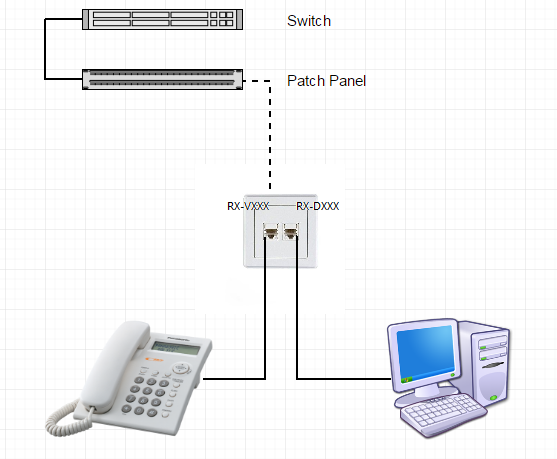
\includegraphics[scale=1.1]{area_trabajo.png}
\end{center}
	
	\chapter{Justificaciones}
\section{Cableado horizontal}
Los Rack de ambas plantas se han colocado en las salas informáticas ya habilitadas, las cuales tienen espacio suficiente para ellos y son también una localización lógica, por razones como seguridad tanto contra intrusiones(ya que solo el personal autorizado tendrá acceso a esta salas) como ambientales (se puede mantener la temperatura adecuada para ellos sin afectar al resto del personal). Están además a suficiente distancia de fuentes de interferencias como pueden ser los ascensores. Desde estas salas se cumplen también los criterios de distancia máxima para el entramado de conexión horizontal del estándar IEEE 802.3

Se han elegido cables categoría 7a, permitiendo la implantación de una red 10 Gigabit Ethernet de hasta 10Gb/s. La red de cableado se ha distribuido por el falso techo, de forma que no supongan ningún estorbo para los trabajadores y permitiendo una distribución más flexible, que podría cambiarse fácilmente si se diera la necesidad.

Las rosetas de conexión constan de 4 puertos (3 de datos y uno de voz) de forma que se pueda dedicar uno para dispositivos como teléfonos (pudiéndose usar uno de datos si el de voz fallara) y permitiendo la conexión simultánea de 3 dispositivos que necesiten acceder a la red, o pudiendo mantener conectado el dispositivo más vital en caso de fallos de algunos de los puertos, hasta que estos se arreglaran.

Hay colocados varios puntos de acceso inalámbricos en zonas donde puedan ser necesarios donde por lo general prevalecen dispositivos como móviles o tabletas. Entre ellas, salas amplias donde la cercanía de conexiones físicas puede ser un problema, salas alejadas de puestos de trabajo donde no se necesita gran velocidad de transferencia de datos, o salas de reuniones donde tampoco se necesite gran velocidad de transferencia y se quiera evitar el uso de cables por comodidad.

El etiquetado usado en el cableado horizontal ya ha sido explicado con anterioridad en el capítulo 1 de este documento.
\section{Distribuidores}
Hemos elegido los siguientes elementos para nuestro Racks debido a varias causas. Empezaremos describiendo el Rack de la planta baja, etiquetado como ``Rack 0'' y luego el Rack de la planta alta, etiquetado como ``Rack 1''.
\subsection{RACK 0}
En este rack, hemos incorporado cinco switches CISCO Catalyst 2960S para poder abarcar todos los paneles de datos que se encuentran en dicha planta. El quinto switch queda para la conexión entre el Rack 0 y el Rack 1 mediante fibra óptica. Sus 48 puertos restantes quedan por si queremos realizar una ampliación del cableado en un futuro.

Adicionalmente, dichos switches tienen PoE (Power Over Ethernet); de forma que los mencionados switches pueden proveer corriente eléctrica mediante los cables de la red Ethernet.

El etiquetado para cada switch será de tipo \textbf{SW-X-R0}; donde ‘X’ corresponde al número del switch. A su vez cada swtich irá etiquetado con los paneles de datos correspondientes a los que proporciona red. Los switches irán conectados entre sí mediante fibra óptica multimodo.

El router (CISCO 2811), etiquetado como RE también cuenta con tecnología PoE y cuenta con dos conexiones de fibra óptica para ser conectado al primer switch y al ISP.

Los paneles de parcheo correspondientes a datos son cuatro; de forma que son equivalentes al número de switches usados por los hosts; y por lo tanto también son iguales el número de puertos, cuarenta y ocho. El etiquetado será de tipo \textbf{R0-DXXX – R0-DYYY}; siendo ‘XXX’ el puerto inicial e YYY el puerto final correspondiente a cada panel de parcheo.

En cuanto a la voz, contamos con dos paneles de parcheo de voz para abarcar todos los dispositivos de teléfono VoIP que se encuentran en la planta baja.

Para darle señal telefónica a ambas plantas contamos con una centralita telefónica Nexspan A5000 2XS; que cuenta con 112 puertos, que son pocas más de las que necesitamos para que todos nuestros teléfonos VoIP funcionen correctamente.

Contamos con un SAI Lapara Serie On-Rack (UPS) para prevenir perder datos si la corriente eléctrica falla (y con ello que el Rack se apague). De esta forma, tendremos un plazo de tiempo para guardar todos nuestros datos y/o  configuraciones de la red.

\subsection{RACK 1}
En el Rack 1, debemos tener en cuenta que el etiquetado funciona de la misma forma que en el Rack 0, y que los modelos usados son los mismos.  Con esto:
\begin{itemize}
	\item Contamos con cuatro switches en lugar de cinco. Todos están conectados en serie al router del Rack 0 de planta baja.
	\item El número de paneles de parcheo de datos corresponde al de número de switches que hay en el Rack 1 usados por los hosts, por lo tanto, hay tres.
	\item Contamos con un panel de parcheo de voz para abarcar todos los teléfonos VoIP que hay en planta.
\end{itemize}

\section{Cableado vertical}
Para la conexión entre los distribuidores de ambas plantas utilizamos fibra óptica multimodo, que es ideal para la comunicación en distancias cortas como las de un campus, o el edificio que nos ocupa, con ello disfrutamos de las ventajas que ofrece la fibra sobre el cableado de cobre, como son una mayor velocidad de transmisión, mayor ancho de banda, inmunidad a interferencias, menor peso y tamaño…

Usamos concretamente cableado OM4, que permite el uso del estándar 10 Gigabit Ethernet hasta una distancia máxima aproximada de 500 metros y llega a soportar conexiones de hasta 125 metros con ratios de 40 a 100 Gbps.\\
En cuanto a presupuesto, la fibra es una opción rentable, con un precio no mucho mayor por metro que la mayoría de cables UTP de categoría 5 o 6.

Los switches de cada rack están conectados entre ellos formando una topología en anillo, lo cual proporciona redundancia para recuperación de fallos (failover).

\section{Plano de conexión}
Tal como se muestra en la imagen del plano de conexión tenemos un cable categoría 7a que va desde el patch panel hasta la roseta de pared del puesto de trabajo.

En dicho puesto, contamos con cuatro conexiones rj45, tres de datos y una de voz, donde usamos el etiquetado que comentamos en el apartado del cableado horizontal. El cableado que va desde la roseta hasta el host es también categoría 7a.

La decisión de contar con tres tomas de datos en el puesto de trabajo surge de la posibilidad de la existencia de una avería en cualquiera de las tomas que se estén usando actualmente o para la ampliación de dicho puesto de trabajo.
	\newpage
	\textcolor{White}{ }
%	\chapter{Plano completo}
\end{document}


